%%%%%%%%%%%% 选择学位类型:学博%%%%%%%%%%
%%% 单面论文
% \documentclass[AcMaster]{BJTU-thesis}  
%%% 双面论文
\documentclass[Doctor,twoside]{BJTU-thesis}
%%EnMaster专硕
%%AcMaster学硕
%%Doctor学博

%%%%%%%%%%%%%%%%%%%     字体     %%%%%%%%%%%%%%%%%%%%%
\setmainfont{Times New Roman}
\setCJKmainfont{SimSun}  				   %%% Overleaf 和 TexStudio 字体库不同,使用Overleaf时请注释


% 标题宋体加粗问题
\setCJKfamilyfont{zhsong}[AutoFakeBold = {2.17}]{SimSun}   %%% Overleaf 和 TexStudio 字体库不同,使用Overleaf时请注释
\renewcommand*{\songti}{\CJKfamily{zhsong}}                %%% Overleaf 和 TexStudio 字体库不同,使用Overleaf时请注释


%%%%%%%%%%%%%%%%%%%    导入包    %%%%%%%%%%%%%%%%%%%%%
% Table
\newlength\savewidth 
\newcommand\shline{\noalign{\global\savewidth\arrayrulewidth\global\arrayrulewidth 1.2pt}\hline
                   \noalign{\global\arrayrulewidth\savewidth}}
\newcommand{\tablestyle}[2]{\setlength{\tabcolsep}{#1}\renewcommand{\arraystretch}{#2}\centering\fontsize{10pt}{12pt}\selectfont}
\newcommand{\smalltablestyle}[2]{\setlength{\tabcolsep}{#1}\renewcommand{\arraystretch}{#2}\centering\fontsize{8pt}{10pt}\selectfont}

% other
\usepackage{pifont}
\usepackage[ruled]{algorithm2e} 
% 设置算法环境的关键字为中文
\renewcommand{\algorithmcfname}{\songti\textbf{算法}} % 修改algorithm环境的标题
\renewcommand{\KwIn}{\songti\textbf{输入: }} % 修改Input关键字
\renewcommand{\KwOut}{\songti\textbf{输出: }} % 修改Output关键字



%%%%%%%%%%%%%%%%%填写封面信息%%%%%%%%%%%%%%%%%%%%%%%%
\author{}  %作者姓名
% \author{}  %mis 13处修改(cls有一处)
\studentNumber{20}  %作者学号
% \studentNumber{}  %mis
\advisor{}  %导师姓名
% \advisor{}  %mis
\advisorTitle{教授} %导师职称
\degreeType{工学}  %学位类别
\major{交通信息工程及控制}  %所属专业
% \major{}  %mis
\researchArea{图像处理与模式识别}  %研究方向
% \researchArea{}  %mis
\title{面}  %论文题目
\englishtitle{Research }  %论文题目英文
\datetime{2024年6月}  %编辑日期


%%%%%%%%%%%%%%%%%%%%%%%   单双页   %%%%%%%%%%%%%%%%%%%%%%%%%%
% 插入空白页
\usepackage{afterpage}
\newcommand\myemptypage{
    \newpage\thispagestyle{empty}\null
    % \addtocounter{page}{-1}
    \newpage
}

% 解决双面包括封面的问题,被包含的内容不分奇偶
\makeatletter
\newcommand{\openany}{\@openrightfalse}
\newcommand{\openright}{\@openrighttrue}
\makeatother

% twoside解决拉长段落间距问题
\raggedbottom

\begin{document}

     %%%%%%%  被包含的内容不分奇偶  %%%%%%%%%%%%
     \openany
	\makecover
     % 空白页1
     \myemptypage

     % 版权
	% \makeAuthorization
     %版权授权袁雪书

\chapter*{学位论文版权使用授权书}
\thispagestyle{empty}
本学位论文作者完全了解北京交通大学有关保留、使用学位论文的规定。特授权北京交通大学可以将学位论文的全部或部分内容编入有关数据库进行检索,提供阅览服务,并采用影印、缩印或扫描等复制手段保存、汇编以供查阅和借阅。同意学校向国家有关部门或机构送交论文的复印件和磁盘。学校可以为存在馆际合作关系的兄弟高校用户提供文献传递服务和交换服务。

(保密的学位论文在解密后适用本授权说明)


\vspace{72pt}
学位论文作者签名:~~~~~~~~~~~~~~~~~~~~~~~~~~~~~~~~~~~~~~导师签名:
	
\vspace{12pt}
签字日期:~~~~~~~~~~~年~~~~~~~~月~~~~~~~~日~~~~~~~~~~~~~~~~~签字日期:~~~~~~~~~~~~年~~~~~~~~月~~~~~~~~日 


% 签名版
% 学位论文作者签名:~\hspace{0.2em}\raisebox{-6pt}{\includegraphics[height=1.4\baselineskip]{figures/xxx电子签名.png}}~~~~~~~~~~导师签名:~\hspace{0.1em}\raisebox{-10pt}{\includegraphics[height=1.9\baselineskip]{figures/电子签名.jpg}}

% \vspace{12pt}
% 签字日期:~\hspace{0.2em}\raisebox{-10pt}{
\includegraphics[height=1.5\baselineskip]{figures/时间2024.png}}年~\hspace{0.2em}\raisebox{-3pt}{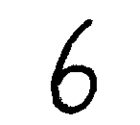
\includegraphics[height=1.0\baselineskip]{figures/时间6.png}}月~\hspace{0.2em}\raisebox{-6pt}{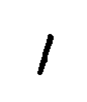
\includegraphics[height=1.2\baselineskip]{figures/时间1.png}}日~~~~~~~~~签字日期:~\hspace{0.2em}\raisebox{-10pt}{
\includegraphics[height=1.5\baselineskip]{figures/时间2024.png}}年~\hspace{0.2em}\raisebox{-3pt}{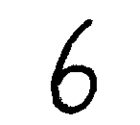
\includegraphics[height=1.0\baselineskip]{figures/时间6.png}}月~\hspace{0.2em}\raisebox{-6pt}{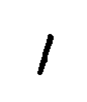
\includegraphics[height=1.2\baselineskip]{figures/时间1.png}}日





 	%版权
     % 空白页2
     \myemptypage

     % 内封
	\makeInfo
     % 空白页3
     \myemptypage

     \begin{committee}


\begin{center}
    % \bigskip % 添加一些垂直空间

    % 增加行高
    \renewcommand{\arraystretch}{2}

    % 创建一个新的列类型,命名为 'M',它会创建一个宽度和垂直居中的居中列
    \newcolumntype{M}[1]{>{\centering\arraybackslash}m{#1}}
    
    \begin{center}
    \begin{tabular}{ | M{2.5cm} | M{2.5cm} | M{5cm} | M{3cm} | }
    \hline
    \songti\textbf{答辩委员会} & \songti\textbf{姓名} & \songti\textbf{工作单位} & \songti\textbf{职称} \\
    \hline
    主席 &  & 北京理工大学 & 教授 \\
    \hline
    委员 &  & 大学 & 教授 \\
    \hline
    委员 &  & 北京交通大学 & 教授 \\
    \hline
    委员 &  & 北京交通大学 & 教授 \\
    \hline
    委员 &  & 北京交通大学 & 教授 \\
    \hline
    秘书 &  & 北京交通大学 & 高工 \\
    \hline
    % ... 其他行
    \end{tabular}
    \end{center}
\end{center}

\end{committee}




 	%答辩委员会名单
     \myemptypage
 
     \begin{thanks}






\end{thanks} 	%致谢部分
     % 空白页4
     \myemptypage
        
     \openright
     %%%%%%%  被包含的内容不分奇偶  %%%%%%%%%%%%
        
	\begin{abstract}

随着技术


% \vspace{\baselineskip}


\noindent\keywords{无人视觉感知系统;跨域自适应}
\end{abstract}  %中文摘要
	\begin{englishabstract}

As 




% \vspace{\baselineskip}

\noindent\englishkeywords{Unmanned visual perception system; Cross-domain adaptive; }
\end{englishabstract}   %英文摘要
     % \begin{preface}
	[鼠标左键单击选择该段落,输入替换之。内容为小四号宋体。] 学位论文的序或前言,一般是作者或他人对本篇论文基本特征的简介,如说明研究工作缘起、背景、主旨、目的、意义、编写体例,以及资助、支持、协作经过等;也可以评述和对相关问题发表意见。这些内容也可以在正文引言中说明。
		
	
\end{preface}  %序言

	
	\tableofcontents
     \newpage\pagenumbering{arabic}
 
        
 
     %正文部分
     \chapter{绪论}
\label{cha:intro}

\section{研究背景与意义}

无人系统~\cite{ZGJX201517001}。此类技术~\cite{stampa2021maturity}。
% --------------------- FIG 1 --------------------#
\begin{figure*}[!htb] 
    \centering
    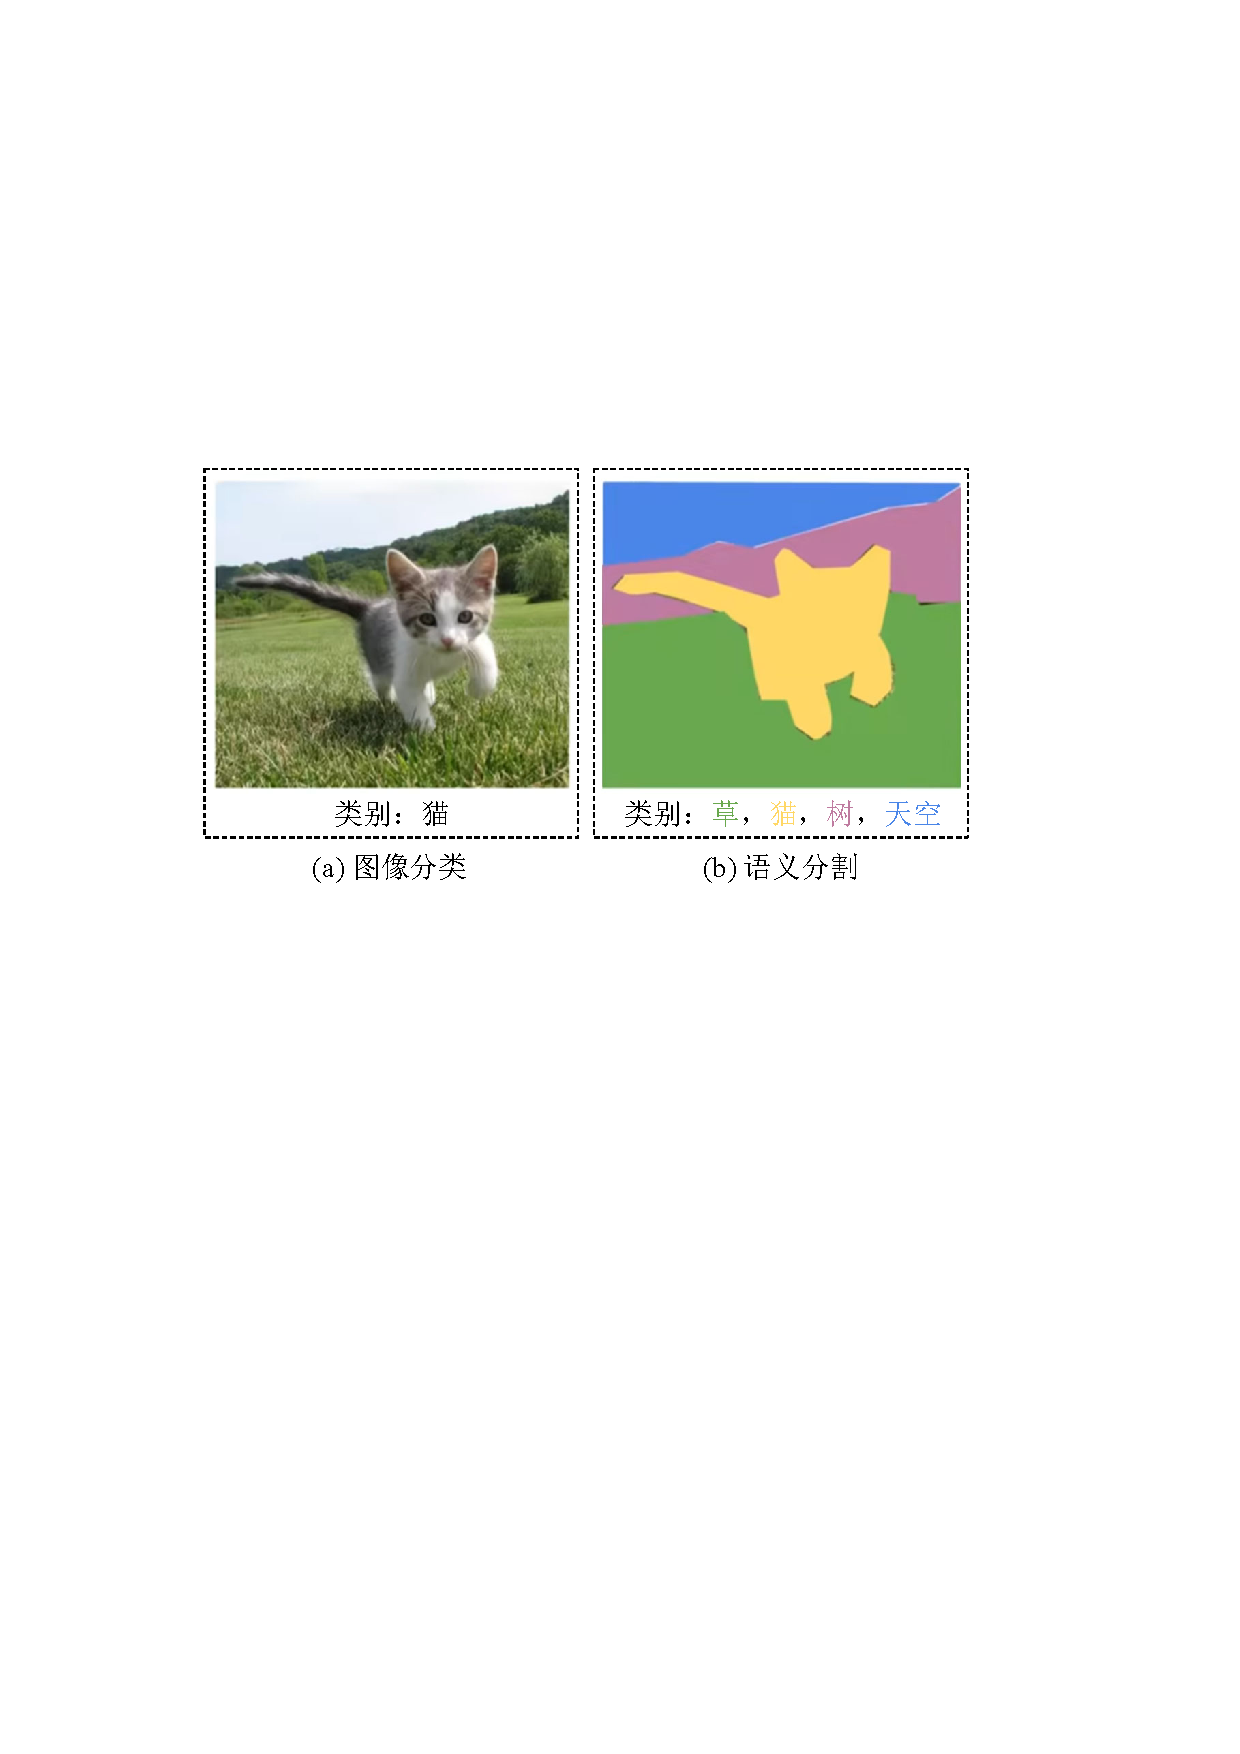
\includegraphics[width=0.66\linewidth]{figures/c01/Fig1.pdf}
    \caption{图像分类与语义分割}
    \vspace{-4mm}
    \caption*{Fig.~\ref{fig_01_01}~Image classification and semantic segmentation}
    \label{fig_01_01}
\end{figure*}
% --------------------- FIG 1 --------------------#

\songti\textbf{(2)语义分割技术的研究现状}
 	%引言
     \chapter{相关知识概述}
\label{cha:chap2}



 	%第二章
     \chapter{基于}
\label{cha:chap3}

计算过程见式(\ref{equ_03_01}):
% --------------------- EQU 1 --------------------#
\begin{equation}
    AP=\mathrm{A}(\emph{IS}_{\bm{\bm{\theta}}}, \mathcal{D}^{u})
   \label{equ_03_01}
\end{equation}
% --------------------- EQU 1 --------------------#



如表 \ref{tab_03_01} 所示

% --------------------- TAB 1 --------------------#
\begin{table*}[!thp]
    \caption{``汽车"精度预测对比实验结果}
    \vspace{-4mm}
    \caption*{Table~\ref{tab_03_01}~Comparative experiment result of the ``car" accuracy prediction}
    \label{tab_03_01}
    \tablestyle{2.0pt}{1}
    \begin{tabular}{c|c|cc|cc|cl}
        \shline
        测试组集 & 真实精度(\%) &\multicolumn{2}{c|}{弗雷歇距离} &\multicolumn{2}{c|}{预测精度(\%)} &\multicolumn{2}{c}{均方根误差} \\
        \hline
        - &汽车 &对比方法 \cite{deng2021labels} &本章方法  &对比方法 \cite{deng2021labels} &本章方法   &对比方法 \cite{deng2021labels} &本章方法   \\
        \hline
        1 &25.98 &123.32 &40.11 &32.62 &\textbf{29.19} &\multirow{18}{*}{6.48} &\multirow{18}{*}{\textbf{2.35}} \\
        2 &19.15 &154.79 &52.47 &26.57 &\textbf{21.01} & & \\ 
        3 &26.00 &134.26 &39.84 &30.52 &\textbf{29.36} & & \\
        4 &45.29 &90.17 &19.48 &38.99 &\textbf{42.83} & & \\
        5 &41.78 &115.89 &15.40 &34.05 &\textbf{45.53} & & \\
        6 &42.93 &119.15 &14.15 &33.42 &\textbf{46.35} & & \\
        7 &20.98 &136.86 &50.21 &30.01 &\textbf{22.50} & & \\
        8 &16.88 &160.22 &55.74 &25.52 &\textbf{18.85} & & \\
        9 &43.87 &113.63 &15.34 &34.48 &\textbf{45.57} & & \\
        10 &30.98 &117.66 &33.34 &33.71 &\textbf{33.66} & & \\
        11 &33.20 &130.36 &31.28 &31.27 &\textbf{35.02} & & \\
        12 &27.24 &141.87 &39.67 &\textbf{29.05} &29.47 & & \\
        13 &50.64 &70.40  &9.50  &42.79 &\textbf{49.43} & & \\
        14 &28.28 &112.67 &38.72 &34.67 &\textbf{30.10} & & \\
        15 &26.90 &126.24 &42.56 &32.06 &\textbf{27.56} & & \\
        16 &27.28 &135.94 &47.92 &\textbf{30.19} &24.02 & & \\
        17 &32.78 &120.58 &33.71 &\textbf{33.15} &33.42 & & \\
        18 &44.47 &98.59  &18.83 &37.37 &\textbf{43.26} & & \\
        \shline
    \end{tabular}
\end{table*}
% --------------------- TAB 1 --------------------#

 	%第三章
     \chapter{基于}
\label{cha:chap4}

第 \ref{cha:chap3} 章


 	%第四章
     \chapter[基于有效操作的标记成本计算及加权不确定性的主动域适应实例分割]{基于有效操作的标记成本计算及加权不确定性的主动\\域适应实例分割}
\label{cha:chap5}

算法 \ref{algo_04_01} 更加清晰地展示了加权不确定性样本选择策略的流程。
% --------------------- Algo 1--------------------#
\begin{algorithm} 
    \small
    \caption{加权不确定性样本选择流程}  
    \label{algo_04_01}
    \KwIn {实例分割检测器$\emph{ISD}$\\
    \qquad \quad 未标记的目标域 $\mathcal{D}_T$\\
    \qquad \quad 总的标记预算 $L$\\}
    \KwOut {最有助益的样本}

    \For {$x_{i} \in D_{T}$} {
       {根据\\}
    }
    \For {$j_{i} \in S_{U}$} {
        \If {$l\leq L$} {
            {选择样本 $j_{i}$;\\}
            {更新标记成本 $l++$;\\}
        }
    }  
\end{algorithm} 
% --------------------- Algo 1--------------------#
 	%第五章
     \chapter{基于}
\label{cha:chap6}

 	%第六章
     \chapter{结论与展望}
\label{cha:chap7}


 	%第七章

	% \nocite{*}
         
	\bibliography{reference/ref}  %参考文献
     \myemptypage

     \backmatter

     % 附录
	% \begin{appendix}
	% 	%%% Local Variables:
%%% mode: latex
%%% TeX-master: "../main"
%%% End:


\chapter{附录A}

%\section*{附录标题}
%\zihao{5}
%[内容为五号宋体。] 附录是作为论文主体的补充项目,并不是必须的。
%论文的附录依序用大写正体英文字母A、B、C……编序号,如:附录A。
%\vspace{0.75cm}
\begin{center}
\zihao{3}
\textbf{附录标题}
\end{center}



\indent
\zihao{5}
[内容为五号宋体。] 附录是作为论文主体的补充项目,并不是必须的。
论文的附录依序用大写正体英文字母A、B、C……编序号,如:附录A。
	% \end{appendix}

    % 索引
     % %%% Local Variables:
%%% mode: latex
%%% TeX-master: "../main"
%%% End:


\chapter{索引}



\indent
\zihao{5}
[内容为五号宋体。] 按照需要编排分类索引、著者索引、关键词索引等。 	


	%\mmchapter{作者简历}
\chapter{作者简历及攻读博士学位期间取得的研究成果}\zihao{5}
\setlength{\parindent}{0pt}

%[内容采用五号宋体]  包括教育经历、工作经历、攻读学位期间发表的论文和完成的工作等。行距16磅,段前后各为0磅。

一、作者简历

%mis
\songti\textbf{教育经历:}  

\vspace{-0.7\baselineskip} % 减少前后间距但不是完全移除

\begin{tabbing}
    2020年9月-至今 \hspace{2cm} \= 北京交通大学自动化与智能学院 \hspace{2cm} \= 攻读博士学位 \\
    2017年9月-2020年6月 \> 大学学院 \> 攻读硕士学位 \\
    2013年9月-2017年6月 \> 大学学院 \> 攻读学士学位 \\
\end{tabbing}
\vspace{-1.2\baselineskip} % 减少前后间距但不是完全移除
    
\songti\textbf{所获奖励:}
\vspace{-0.6\baselineskip} % 减少前后间距但不是完全移除
\begin{tabbing}
    2022-2023年度 \hspace{1cm} \=  北京交通大学 \hspace{2.8cm} \= 奖学金 \\
\end{tabbing}
\vspace{-0.7\baselineskip} % 减少前后间距但不是完全移除


二、发表论文

[1] \textbf{xxx}, 




\vspace{10pt}
三、参与科研项目

%mis
[1] 国家自然科学基金``面上"项目:复杂


\vspace{10pt}



四、专利

%mis
[1] 





%\section*{访学经历}
%2011年8月至2011年11月,访问XX大学XX系,合作导师:XX教授;
%
%\section*{承担的科学研究工作}
%  (1) 主持,XX项目...。
%
%  (2) 参加,...;
%
%
% \section*{获奖情况}
   


  %作者简历
     \myemptypage

     \chapter{博士论文答辩决议}\zihao{5}

\hspace{2em}论文

\hspace{2em}1. 

\hspace{2em}2. 

\hspace{2em}3. 

\hspace{2em}4. 

\hspace{2em}

\hspace{2em}论文工作表明作者已掌握了本学科坚实宽广的基础理论和系统深入的专门知识,具有独立从事科研工作的能力。答辩过程中讲述清楚,回答问题正确。

\hspace{2em}答辩委员会经无记名投票,一致同意通过xxx博士学位论文答辩,并建议授予工学博士学位。












  %博士论文答辩决议
     \myemptypage

	\chapter{独创性声明}


\zihao{5}

 
\hspace{2em}本人声明所呈交的学位论文是本人在导师指导下进行的研究工作和取得的研究成果,除了文中特别加以标注和致谢之处外,论文中不包含其他人已经发表或撰写过的研究成果,也不包含为获得北京交通大学或其他教育机构的学位或证书而使用过的材料。与我一同工作的同志对本研究所做的任何贡献均已在论文中作了明确的说明并表示了谢意。



\vspace{72pt}
 
\hspace{2em}学位论文作者签名:~~~~~~~~~~~~~~~~~~~~~~~~~~~~~~~~~~~~~~~~~~~签字日期:~~~~~~~~~~~~年~~~~~~~~月~~~~~~~~日 




% 签名版
% \hspace{2em}学位论文作者签名:\hspace{0.2em}\raisebox{-6pt}{\includegraphics[height=1.4\baselineskip]{figures/电子签名.png}}~~~~~~~~~~~~~~~~~~~~签字日期:~\hspace{0em}\raisebox{-9pt}{
\includegraphics[height=1.5\baselineskip]{figures/时间2024.png}}年~\hspace{0.1em}\raisebox{-3pt}{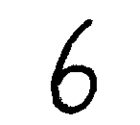
\includegraphics[height=0.9\baselineskip]{figures/时间6.png}}月~\hspace{0.1em}\raisebox{-6pt}{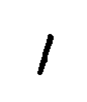
\includegraphics[height=1.2\baselineskip]{figures/时间1.png}}日



 	%独创性声明
     \myemptypage
 
     
\chapter{学位论文数据集}\zihao{5}



\setcounter{table}{0}
\renewcommand{\thetable}{1.\arabic{table}}

\begin{table}[!h]

\small 
\centering
\caption{数据集页}
\begin{tabular}{|p{2.6cm}|p{2.6cm}|p{2.5cm}|p{2.9cm}|p{2.5cm}|}
\hline
%\multirow{2}{*}{1} & \multicolumn{2}{|c|}{1} \\
%\cline{2-3}
%& 1 & 1 \\
%\hline
%1 & \multicolumn{2}{|c|}{1}\\
关键词$^*$  & 密级$^*$ & 中图分类号 & UDC & 论文资助 \\
\hline
    无人;跨域;    &公开   & TP391           &     &          \\  %对应上一行的标题对应填写: 关键词、密级、中图分类号、UDC、论文资助
\hline

\multicolumn{2}{|p{5.4cm}|}{学位授予单位名称$^*$} & 学位授予单位代码$^*$ & 学位类别$^*$ &  学位级别$^*$    \\
\hline
\multicolumn{2}{|p{5.4cm}|}{北京交通大学 }        &  10004               &工学              &博士         \\%对应上一行的标题对应填写: 学位类别、学位级别
\hline

\multicolumn{2}{|p{5.4cm}|}{论文题名$^*$} & \multicolumn{2}{p{5.4cm}|}{并列题名} &  论文语种$^*$    \\
\hline
\multicolumn{2}{|p{5.4cm}|}{面向研究}  & \multicolumn{2}{p{5.4cm}|}{ }        &中文      \\ %对应上一行的标题对应填写: 论文题目、并列题名、论文语种
\hline

\ 作者姓名$^*$    &  \multicolumn{2}{p{5.4cm}|}{}   & 学号$^*$  &20     \\%在对应空格上填写:作者姓名,学号 
% \ 作者姓名$^*$    &  \multicolumn{2}{p{5.4cm}|}{}   & 学号$^*$  &     \\%mis
\hline

\multicolumn{2}{|p{5.4cm}|}{ 培养单位名称$^*$ }  &  培养单位代码$^*$   & 培养单位地址  &  邮编   \\
\hline
\multicolumn{2}{|p{5.4cm}|}{北京交通大学}  &  10004   & 北京市海淀区西直门外上园村3号  & 100044   \\
\hline

\multicolumn{2}{|p{5.4cm}|}{ 学科专业$^*$ }  &  研究方向$^*$   & 学制$^*$  & 学位授予年$^*$   \\
\hline
\multicolumn{2}{|p{5.4cm}|}{交通信息工程及控制}  &图像处理与模式识别    &四年        & 2024     \\%对应上一行的标题对应填写:学科专业、 研究方向、学制、学位授予年
% \multicolumn{2}{|p{5.4cm}|}{}  &    &四年        & 2024     \\%mis

\hline
论文提交日期 $^*$    & \multicolumn{4}{c|}{2024年06月}   \\%在对应空格上填写:论文提交日期 
\hline

\ 导师姓名$^*$    &  \multicolumn{2}{p{5.4cm}|}{}   & 职称$^*$  &教授     \\%在对应空格上填写: 导师姓名、职称
% \ 导师姓名$^*$    &  \multicolumn{2}{p{5.4cm}|}{}   & 职称$^*$  &教授     \\%mis
\hline

\ 评阅人    &  \multicolumn{2}{p{5.4cm}|}{ 答辩委员会主席$^*$ }   & \multicolumn{2}{p{5.4cm}|}{ 答辩委员会成员$^*$ } \\
\hline
\        &  \multicolumn{2}{p{5.4cm}|}{   }   & \multicolumn{2}{p{5.4cm}|}{   } \\%对应上一行的标题对应填写:评阅人、主席、成员
\        &  \multicolumn{2}{p{5.4cm}|}{}   & \multicolumn{2}{p{5.4cm}|}{ \quad  \quad  \quad } \\
\        &  \multicolumn{2}{p{5.4cm}|}{}   & \multicolumn{2}{p{5.4cm}|}{   } \\

\hline
\multicolumn{5}{|p{13.1cm}|}{ 电子版论文提交格式 \; 文本( $\surd$ )  图像( ) 视频( ) 音频( ) 多媒体( ) 其他( )}  \\
\multicolumn{5}{|p{13.1cm}|}{ 推荐格式:application/msword; application/pdf }  \\

\hline
\multicolumn{2}{|p{5.4cm}|}{ 电子版论文出版(发布)者  } & \multicolumn{2}{p{5.4cm}|}{电子版论文出版(发布)地  } & 权限声明\\
\hline
\multicolumn{2}{|p{5.4cm}|}{   } & \multicolumn{2}{p{5.4cm}|}{   } &  \\ %对应上一行的标题对应填写: 电子版论文出版(发布)者、发布地

\hline
论文总页数 $^*$    & \multicolumn{4}{c|}{}   \\%在对应空格上填写:页数
\hline
\multicolumn{5}{|p{13.1cm}|}{ 共33项,其中带$*$为必填数据,为22项。 }  \\



\hline 
\end{tabular}	
\end{table}





















  %学位论文数据集					


\end{document}




















